%chapter 3
\chapter{Transport Economics}
%
\section{Introduction}
All decisions related to planning, design, and improvement of transportation infrastructure have economic implications. Transport economics includes the issues such as transport location, movement of people and freight/goods, transport demand, transport planning and forecasting, direct and indirect cost of transport, pricing of transport services, investments in transport infrastructure and services, transport and social-economic development, and transport regulation. In this chapter the transport economics is considered from the micro economic perspective. We consider various aspects of the direct costs and pricing of transport infrastructure and services of different transportation modes.\\
\par
Considered from this microeconomic perspective, it can be said that the transport sector consists of the demand and supply component. The transport demand is derived demand due to needs of people and freight/goods shipments to change the physical place. For example, many people live at one place but work and/or have a leisure on the others, which requires them to travel forward and backward. The location of companies providing raw materials is different than those of the users of these materials—manufacturers of the semifinal and final products, which requires transportation of these raw materials from the former to the latter. In addition, the manufacturers of the final products are often located far away from the retailers of these products, which again require transportation, this time of the final products. Thus, it can be said that the transport demand is derived demand. In many cases transportation demand is proportional to the volumes of peoples’ activities and the quantities of final products they consume during a given period of time.\\
\par
The transport demand is handled by the transport supply/capacity provided by transport companies.
The transport companies generally provide transport infrastructure with the supportive facilities and equipment, and rolling stock/vehicles carrying out transport services. In order to make them operational, the corresponding material, labor, ie, employed staff/personnel, and energy/fuel, are consumed. In terms of time, the transport infrastructure has particularly the long life-cycle, which is, for example, about 20, 30, 40, or even 60 years. That of rolling stock/vehicles is shorter (20–25 years) mainly due to its/their physical and also technological obsolescence, after they need to be replaced. In this context, two categories of transport companies can be distinguished: that providing transport infrastructure called “the infrastructure providers,” and that providing transport services called “transport operators.” They both constitute the transport systems within particular transport modes.\\
\par
According to the economic jargon, the above-mentioned components of transport supply/capacity represent the main inputs to transport processes. The outputs of the transport process are the transport services produced in the given quantities and at the specified quality. They are consumed by users— passengers and/or freight shippers/receivers at the same time as they are produced. This implies that they are the short-lived similarly as transport demand without possibility to be stored/warehoused and left to be consumed sometimes latter on.\\
\par
The most important economic categories of a given transport system are its costs, revenues, and their relationship.\\
\par
The costs are expenses for maintaining the transport infrastructure and carrying out transport
services. These costs are passed to users of these services (passengers and freight/goods shippers and receivers) in the form of prices/charges. These charges bring revenues to transport companies. In general, these prices/charges, ie, revenues, are set up to cover the company’s costs and provide some profits. Nevertheless, the difference between revenues and costs can generally be positive or negative, thus representing the profits or losses. Profits or losses are calculated for the given period of time (usually for a quarter of year, year, or few years).\\
\par
The prices charged to users of transport services represent for them direct costs. In addition, users are imposed the indirect costs, which are usually considered to be the cost of time during trip/travel/ transportation. In such case, the sum of direct and indirect costs is called the users’ generalized trip/ travel/transportation costs for users.\\
\par
We describe in this chapter the main elements of economics of transportation systems considered
from the engineering perspective. The chapter analyzes direct costs and revenues of the providers of transport infrastructure and transport operators. Costs and revenues could be analyzed at the level of the individual component (infrastructure, rolling stock) and/or of the entire company.
\section{Some Important Terminologies}
\subsection{Transport Industry/Sector}
The transport sector of a specific region continent consists of transport companies providing transport infrastructure (infrastructure providers), and transport services (transport operators). They both could be fully public, fully private, and mixed public/private owned. The transport infrastructure providers obtain investments for building transport infrastructure usually from the national and international banks and monetary funds. Some of the well-known funds are International Monetary Fund, World Bank, and European Central Bank. The obtained investments are usually long-term credits, and they are spread over the life-cycle ofthe given infrastructure. The annuities on the loan, as well as the cost ofcurrent and capital maintenance, are covered by charging transport operators for using the infrastructure. On one hand, these charges represent the revenues ofthe infrastructure providers. On the other hand, they represent the part of the transport operators’ operating costs. The charges enable entry of particular transport operators to the particular link/line/route, node, or a part of the infrastructure network. In general, more than one operator could be allowed to use the transportation infrastructure. This depends on the expected demand volumes, as well as on the capacity ofthe related infrastructure elements. Such policy ofaccess enables competition between different operators, which in general reduces prices charged to their users (passengers and freight/ goods shippers and receivers). For examples, road users—cars, buses, and trucks pay for accessing and use highways, the railway operators are charged for using the rail infrastructure after their separation, ships are charged for accessing ports, airlines pay fees for getting slots at airports, etc.
%
\subsection{Fixed and Variable Costs}
Each transport system is characterized by internal costs and external costs. Internal costs are paid exclusively by the transportation system users. Internal costs are construction costs, maintenance costs, fuel costs, etc. The main external costs are air pollution, high level of noise, negative outcomes on wetlands, negative effects on wildlife habitat, and low water quality. These external costs are paid by the whole society.\\
\par
The total costs of transport infrastructure providers, or transport operators can be divided into two main categories: fixed costs and variable costs.\\\\
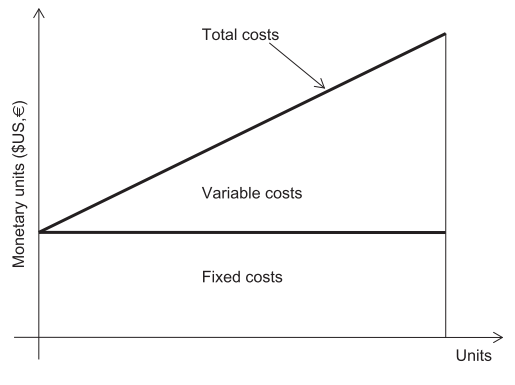
\includegraphics{gfx/fig11.png}\\
The variable costs, that depend on the level of utilization of a given rolling stock/vehicle fleet. They include costs of labor, material, and energy/fuel. These costs are not inevitable. They are lower with the lower utilization of a given rolling stock/vehicle fleet.\\
\par
The total costs $TC(k)$ of any transport company represent the sum of fixed and variable costs, i.e.
\begin{equation}
	\label{total cost}
	TC(k) = FC(k) + VC(k)
\end{equation}
%
Where,\\
\hspace*{10mm}$k$ is the period of time (day, month, quarter, year)\\
\hspace*{10mm}$FC(k)$ is the fixed costs incurred during the time period $k$\\
\hspace*{10mm}$FC(k)$ is the variable costs incurred during the time period $k$\\\\
In addition, the fixed cost of the infrastructure providers and transport operators for construction of infrastructure and acquiring the rolling stock/vehicle fleet are covered by the investments. These, after uniformly spread over the given period of time, usually over the predicted life-cycle, are expected to bring benefits to the actors/stakeholders involved such as investors, transport infrastructure providers and transport operators, users/passengers and freight/goods shippers and receivers, and the local, regional, national, and global community, ie, the economy and society.
%
\subsection{Economies of Scale and Economies of Scope}
The average costs per unit of output are obtained by dividing the total costs (Eq. \ref{total cost}) by the volume of output. The output could be the number of vehicles, the number of passengers, quantity of freight/ goods, the number of vehicle-kilometers, the number of passenger-kilometers, the number of freight-kilometers, etc. If this average cost decreases with increasing of the volume of given output, he economies of scale exist. Otherwise, economies of scope exist. In the former case, in general, the average cost decreases because of spreading the fixed costs over the larger number of units of output. Economies of scale could be interpreted as the cost advantages that companies achieve as a result of size, output, or scale of operations. For example, when the output increases from O1 to O2, the average cost of each unit decreases from AC1 to AC2 as shown in the figure below.\\
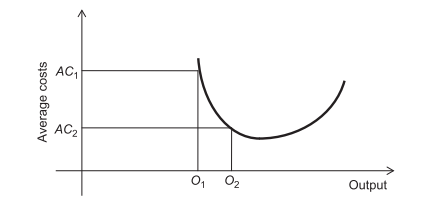
\includegraphics{gfx/fig12.png}\\
Trucking, delivery companies, and airlines usually organize a hub-and-spoke networks as the flows between hubs are characterized by economies of scale. At hubs, goods or passengers are exchanged across vans, trucks, and planes.\\
\par
Based on Eq. \ref{total cost}, the average cost per unit of output can be estimated in the following way:
\begin{equation}
	AC(k) = TC(k)/VO(k) = [FC(k) + VC(k)]/VO(k)
\end{equation}
Where $VO(k)$ is the volume of output during the time period (k) (number, quantity).\\
\par
Transportation projects and transportation operations are also characterized by marginal costs. Marginal costs are defined as the change in total cost caused by supplying an additional unit of transport capacity—transport service, seat at transport service, etc. Marginal costs have a tendency to decrease with transportation project size.\\
\par
Economies of scope are defined as decreasing of the average total cost with increasing of the number of different services produced. In the case of a transport company, this could be offering transport services for both passengers and freight/goods. An airline operating both passenger and cargo aircraft fleet could be an example. Such airline can operate at lower cost than what it would be cost of two separate airlines (one operating passenger aircraft fleet, and the other operating cargo aircraft fleet).\\
\par
\subsection{Revenue}
Revenues are amounts of money that a transport company receives during a specific period of time from charging its transport services to users. These are calculated by multiplying the price at which the given services are sold by their number carried out during the specified period of time.\\
\par
Net income represents the difference between the revenues and costs, which a given transport company or transport sector has achieved during the specified period of time (usually a quarter or a year). It can be estimated as follows:
\begin{equation}
	I(k) = R(k) - C(k)
\end{equation}
%
Where $R(k)$ is the revenues of a transport company achieved during the time period $k$ (In monetary units)\\
\par
This income can be positive (revenues are greater than costs) in which case, after being taxed, represents profits. Otherwise, the negative net income (revenues are lower than costs) represents loses in the given context.\\
\par
Profit margin represents the ratio of net income and total revenues, as follows:\\
\begin{equation}
	PM(k) = I(k)/R(k) = [R(k) - C(k)]/R(k)
\end{equation}
where the other symbols are analogous to those in the previous equations. In effect, as defined above, the profit margin measures how much income a transport company has from each unit of the revenues earned. For example, a 10\% profit margin implies that the company has a net income of €0.10 for each Euro of the total revenues.\\
\subsection{Relationship Between Demand and Supply}
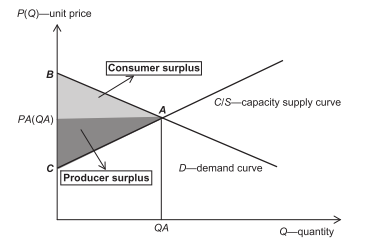
\includegraphics{gfx/fig13.png}\\
Transport companies supply transport capacity to satisfy the expected demand during a given period of time. This is carried out based on the unit price of output/transport service. The unit price is based on the revenues obtained by the given capacity supply and its related costs. In general, when the unit price decreases, the demand for transport services generally tends to increase, and vice versa. Under the same conditions, the total capacity supply and related costs tend to increase, and vice versa. The above figure shows the simplified scheme of the relationship between demand and capacity supply depending of the unit price.\\
\par
Quantity demanded and quantity supplied are the functions of the unit price. The figure shown above does not follow the standard graphical representation of the functions. Traditionally, in economic literature, the unit price is on the vertical axis, and quantity on the horizontal axis.\\
\par
As it can be seen from the above figure, the demand and capacity supply curves intersect at the point A.At this point the quantity demanded $Q_A)$, at the current price $P_A(Q_A)$, is equal to the quantity supplied at the current price $P_A(Q_A)$, resulting in an economic equilibrium.\\
\par
The relationship between the two curves indicates two phenomena: consumer and producer surplus.
The former appears when the users—passengers or freight/goods sippers/receivers are willing to pay the price for service even above its market-balanced level (Triangle: A-$P_A(Q_A)$-B). The latter represents the difference between the amount that a transport company is willing and able to supply and the amount it actually receives by charging its supply at the market-balanced prices (Triangle: A-$P_A(Q_A)$-C). As such, this is considered as the benefit for the transport company operating in the market under given conditions. In addition, the sum of the consumer and producer surplus (Triangle: A-B-C) represents the economic welfare, ie, the utility, which could be gained by both users and producers, ie, suppliers of transport services under given (market) conditions.
%
\section{Transportation Projects Evaluation}
Construction of highways along with the other associated infrastructures, construction of a new freight center, acquisition of new vehicles for the transit e.t.c. represent transportation projects faced by transportation experts. In the initial stage of these projects, it is necessary to perform their evaluation, that is, as precise as possible, analyze and review economic, environmental, equity, as well as other project impacts. The planners and engineers must properly answer the following questions: (a) Are the transportation project’s benefits greater than the projects’ costs?; (b) What is the best project’s alternative in the case when project has few mutually exclusive alternatives?; (c) How to allocate available funds among competitive transportation projects?; (d) When to start the considered project?\\
\par
Frequently, financial resources are scarce, and appropriate engineering economic analysis can significantly help planners and decision-makers to allocate available resources properly. In the first step ofany project evaluation, it is necessary to analyze the project’s socio-economic context, and to clearly define the project’s objectives. In the next steps, the analysts should clearly recognize the type of costs and benefits, compare them and make recommendations to the decision makers.\\
\par
Transportation projects usually extend over many years. On the other hand, the purchasing power of money decreases over time. The main cause of this phenomenon is the inflation that exists in every society. A discount rate regulates the value ofmoney for time. This rate is used to represent future monetary quantities in terms oftheir today’s value. Compounding and discounting are techniques that enable us to compare money values at different points in time. Let us briefly explain compounding technique.\\
\par
Let us assume that we want to invest \$100 these days, at an annual interest rate (r) of 5\%. It will be \$100 + \$5 = \$105 in 1 year. After two years it will be 105\$ + \$0.05 * 105 = \$110.25. After 3 years we will have \$110.25 + \$0.05 * \$110.25 = \$115.7625. Discounting represent reverse operation of compounding. The compounding technique helps us to find the answer to the following question: what is the present value $(PV)$ of a known future amount of money?\\
\par
In our example, the $PV$ of \$105 next year, when $r$ = 5\%, is \$100. The $PV$ equals
\begin{equation}
	PV = V_t/(1 + r)^t \; \; t = 0, 1, 2,......,n
\end{equation}
Where $n$ is the project duration (in years), $r$ is the rate of discount, and $V_t$ is the value in year $t$.\\
\par
There are two interest rates that are used in transportation projects evaluation. The first one is the real interest rate that is exclusive of inflation, while the second one is the nominal interest rate that is inclusive of inflation. Project value is usually expressed as a NPV. This value represents a project’s value or cost for its whole life cycle in today’s dollars.\\
\par
When evaluating transportation projects many governments and funding agencies in the world (OECD, World Bank, etc.) require a cost-benefit analysis (CBA) to be performed. In this way, the CBA represents common evaluation language between the governments, funding agencies and the transportation project supporters.\\
\section{Cost-Benefit Analysis}
The CBA is a method that calculate and compare project’s costs and benefits to society over period of time. The CBA monetizes all project’s inputs and outputs. In other words, the CBA converts the inputs and the outputs into a monetary values. The CBA helps decision-makers to rank and prioritize various project’s alternatives including also alternative “no action” (“no action,” or “do nothing” case assumes continued operation of the existing facility, exclusive of any major investments). The specific transportation project should start only when the CBA clearly shows to the decision makers that the total benefits to society outweigh the total costs. When performing CBA, the analysts enumerate all project’s costs and benefits to society. In the next step, they assign monetary values to costs and benefits, and discount them to a NPV. All costs, as well as all benefits are added into a single number. The transportation project is evaluated by using total costs, and the total benefits values.\\
\par
In the first step of the CBA, it is necessary to identify transportation project’s alternatives to be
evaluated. Alternatives may represent “do nothing” case, rehabilitation of existing facility, construction of a new facility, etc. Transportation projects have consequences over time. The analysts should also define the time period over which the life cycle costs and benefits of all of the alternatives will be calculated.\\
\par
The project’s economic performances are measured by the following indicators:\\
$NPV$: Net Present Value\\
$IRR$: Internal Rate of Return\\
$B/C$: The Benefit-Cost ratio\\\\
The majority of experts consider the NPV as the most important CBA indicator. The NPV is defined in the following way:
\begin{equation}
	NPV = \sum_{t = 0}^{\infty} \frac{B_t - C_t}{(1 + r)^t}
\end{equation}
Where,\\
\hspace*{10mm}$B_t$: Benefits in year $t$\\
\hspace*{10mm}$C_t$: Costs in year $t$\\
\hspace*{10mm}$n$: Project duration (in years)\\
\hspace*{10mm}$r$: interest rate\\
\hspace*{10mm}$t$: year index\\\\
%
Project’sbenefits andcostsare forecast over the project duration.For example,benefits from road investment could be shorter traveling distance, shorter travel time, reduced number of traffic accidents, etc. The road improvement costs could be project design costs, labor costs equipment costs, material costs, etc.\\
\par
The analysts use a $NPV$ to express a project’s worth for its complete life cycle in today’s money value. We see that the $NPV$ decreases in $r$ (interest rate) increases. In case when $NPV > 0$, the project may be accepted. However, when $NPV < 0$, the considered project should be rejected.Finally, when $NPV = 0$, we conclude that the considered project adds no monetary value. The final decision about such transportation project should be based on some additional criteria.\\
\par
The internal rate of return $(IRR)$ is the indicator that also measures the project’s performances. The $IRR$ is the discount rate/interest rate at which the $NPV = 0$. We calculate the $IRR$ by solving the following equation:
\begin{equation}
	\sum_{t = 0}^{\infty} \frac{B_t - C_t}{(1 + IRR)^t} = 0
\end{equation}
%
The average values of the observed $IRR's$ in a sample of investment projects sponsored by the European Union (EU) at the end of the 20th century are approximately equal to 15\% in the cases of roads and highways, 10\% in the cases of railways and underground, and 25\% in the cases of ports and airports.\\
\par
After calculation net benefits $B$ and net costs $C$, the benefit/cost ratio $\left( \frac{B}{C} \right)$ should be also calculated. (Frequently, it is not easy to estimate future costs, and, especially project’s benefits.) The benefit/cost ratio $\left( \frac{B}{C} \right)$ informs us about the improvement in traffic operations (expressed in dollars) per dollar invested.\\
\par
Analysts and engineers usually perform a sensitivity analysis to conclude how sensitive final results are to changes in hypothesis about the costs, benefits, and discount rate.\\
\par
The main weakness of the CBA is that all transportation project benefits are evaluated only in monetary terms. It is very complicated to value all the costs and benefits of transportation projects in monetary terms. In other words, in many situations, social and environmental aspects of the considered transportation projects are not treated adequately. For example, many traffic safety programs, actions and projects involve the prevention of loss of life. The logical and ethical question is how should we value a life saved? A pure economic approach would suggest to us that the value of life is equal to the PV of lifetime earnings. Obviously, there are numerous opponents to such an oversimplified and ethically questioned approach.\\
%
\section{\emph{Numerical Examples:}}
\emph{Example \#1: Selecting a transportation mode}\\\\
An individual is planning to take a trip between the downtown area of two cities, A and B, which are 400 miles apart. There are three options available:
\begin{enumerate}
	\item \textbf{Travel by air:} This trip will involve driving to the airport near city A, parking, waiting at the terminal, flying to airport B, walking to a taxi stand, and taking a taxi to the final destination.
	\item \textbf{Travel by auto:} This trip will involve driving 400 miles through several congested areas, parking in the downtown area, and walking to the final destination.
	\item \textbf{Travel by rail:} This trip will involve taking a cab to the railroad station in city A, a direct rail connection to the downtown area in city B, and a short walk to the final destination.
\end{enumerate}
Since this is a business trip, the person making the trip is willing to pay up to \$25 for each hour of travel time reduced by a competing mode. (For example, if one mode is two hours faster than another, the traveler is willing to pay \$50 more to use the faster mode.) After examining all direct costs involved in making the trip by air, auto, or rail (including parking, fuel, fares, tips, and taxi charges) the traveler concludes that the trip by air will cost \$250 with a total travel time of five hours, the trip by auto will cost \$200 with a total travel time of eight hours and the trip by rail will cost \$150 with a total travel time of 12 hours.
\begin{itemize}
	\item Which mode is selected based on travel time and cost factors alone?
	\item What other factors might be considered by the traveler in making a final selection?
\end{itemize}
\emph{Solution:} Since travel time is valued at \$25/hr, the following costs would be incurred:\\
\begin{gather*}
	Air: 250 + 25 * 5 = \$375\\
	Auto: 200 + 25 * 8 = \$400\\
	Rail: 150 + 25 * 12 = \$450
\end{gather*}
In this instance, the air alternate reflects the lowest cost and is the selected mode. However, the traveler may have other reasons to select another alternative. These may include the following considerations.
\begin{description}
	\item [Safety:]While each of these modes is safe, the traveler may feel “safer” in one mode than another. For example, rail may be preferred because of concerns regarding air safety issues.
	\item [Reliability:] If it is very important to attend the meeting, the traveler may select the mode that will provide the highest probability of an on-time arrival. If the drive involves travel through work zones and heavily congested areas, rail or air would be preferred. If potential air delays are likely due to congestion, flight cancellations, or inclement weather, another mode may be preferred.
	\item [Convenience]: The number of departures and arrivals provided by each mode could be a factor. For example, if the railroad provides only two trains/day and the airline has six flights/day, the traveler may prefer to go by air.
\end{description}
%
\emph{Example \#2: Computing the Toll to Maximize Revenue Using a Supply—Demand Curve}\\\\
A toll bridge carries 5000 veh/day. The current toll is 150 cents. When the toll is increased by 25 cents, traffic volume decreases by 500 veh/day. Determine the amount of toll that should be charged such that revenue is maximized. How much additional revenue will be received?\\\\
\emph{Solution:}Let x the toll increase in cents.
\par
Assuming a linear relation between traffic volume and cost, the expression
for V is\\\\
$V = 5000 - x/25 (500)$\\
The toll is, $T = 150 + x$\\\\
Revenue is the product of toll and volume,
\begin{gather*}
	R = V * T\\
	= (5000 - x/25 * 500)(150 + x)\\
	= (5000 - 20x)(150 + x)\\
	= 750,000 + 2000 - 20x^2
\end{gather*}
For maximum value of x,\\\\
$\frac{dR}{dT} = 0$\\
$20,000 -40x = 0$\\
$\therefore x = 50 cents$\\\\
The new toll is the current toll plus the toll increase.\\
Toll for maximum revenue = $150 +50 = 200cents$\\
The additional revenue, AR
\begin{gather*}
	= V_max *  T_max - V_current * T_current\\
	= {5000 - 50/25 * 500} * 2 - 5000 * 1.5\\
	= 4000 *2 - 7500\\
	= 8000 - 7500\\
	\therefore AR = =\$500
\end{gather*}
\section{Review Problems}



